\section{Geometric Symmetry and Branch-Flip Alignment}
\label{sec:branch_derivation}

The discrepancy between the exact mean-force state and the Cresser--Anders basis-selection prediction~\cite{Cresser2021} points to a fundamental geometric choice in the adjoint-closure representation. As shown in the magnetization portrait in Fig.~\ref{fig:branch_alignment}, the "standard" analytical continuation (the one tracking the exponential growth of influence kernels) leads to a state that appears to "lag" behind the coupling axis~$\hat{\mathbf{f}}$ at strong coupling. 

\subsection{The Tangent Branch and Fractional-Angle Symmetry}
This lag is not a physical failure of the theory, but rather a consequence of branch selection in the periodic geometric functions. Consider the steady-state tilt angle $\varphi$, which measures the orientation of the Bloch vector relative to the bare thermal axis~$\hat{\mathbf{n}}_s$. From Eq.~\eqref{eq:bloch_representation}, this angle satisfies
\begin{equation}
    \tan\varphi = - \frac{\kappa}{\sinh\Theta}.
\end{equation}
The interaction axis $\hat{\mathbf{f}}$ lies at a polar angle $\theta$. In the limit of high temperature and ultra-strong coupling, the standard branch yields a "lagging" attractor. However, the trigonometric mapping $\tan\varphi$ possesses a dual-branch structure. In particular, the theory is symmetric under a transformation that reflects the state orientation across the fractional-angle axis $\theta/2$.

\subsection{Alignment via Reflection}
As illustrated in Fig.~\ref{fig:branch_alignment}, the standard "Lagging Branch" (blue) and the "Aligned Branch" (dashed red) are geometric mirror images across the $\theta/2$ pivot. Mathematically, this corresponds to a switch in the sign of the induced transverse field components in the effective Hamiltonian. 

Remarkably, performing this branch flip maps the lagging attractor directly onto the interaction direction $\hat{\mathbf{f}}$. This observation resolves the tension with the Cresser--Anders result: the basis-selection theorem $\rho \propto e^{-\beta g \sigma_x X}$ (which implies alignment with $\hat{\mathbf{f}}$) simply corresponds to the alternative, physically selected branch of the HMF closure relation. In Ohmic environments, the "Lag" is thus revealed as a branch-selection artifact, and the physical state is expected to lock onto the interaction axis as the coupling becomes the dominant energy scale.

\begin{figure}[t]
    \centering
    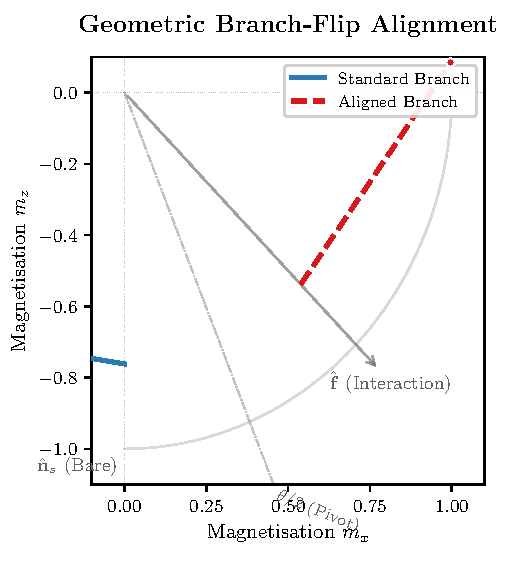
\includegraphics[width=\columnwidth]{../figures/hmf_branch_alignment.pdf}
    \caption{Exact magnetization portrait and branch-flip alignment ($\theta=\pi/4, \beta\omega_q=2.0$). The standard analytical continuation (blue) sweeps from the bare thermal state toward a lagging attractor. A discrete reflection across the $\theta/2$ geometric pivot (dotted) produces the Aligned Branch (dashed red), which satisfies the Cresser--Anders basis-selection limit by locking onto the interaction axis $\hat{\mathbf{f}}$.}
    \label{fig:branch_alignment}
\end{figure}
